\documentclass{article}%
\usepackage[T1]{fontenc}%
\usepackage[utf8]{inputenc}%
\usepackage{lmodern}%
\usepackage{textcomp}%
\usepackage{lastpage}%
\usepackage[head=40pt,margin=0.5in,bottom=0.6in]{geometry}%
\usepackage{graphicx}%
%
\title{\textbf{Saleh: No he dormido sabiendo que siguen inocentes en la celda que estuve}}%
\author{EL NACIONAL WEB}%
\date{14/10/2018}%
%
\begin{document}%
\normalsize%
\maketitle%
\textbf{URL: }%
http://www.el{-}nacional.com/noticias/presos{-}politicos/saleh{-}estoy{-}adaptando{-}libertad{-}fisica{-}realidad{-}calle\_255739\newline%
%
\textbf{Periodico: }%
EN, %
ID: %
255739, %
Seccion: %
Presos políticos\newline%
%
\textbf{Palabras Claves: }%
Oposición, Presos políticos\newline%
%
\textbf{Derecho: }%
1.2, %
Otros Derechos: %
1.1, %
Sub Derechos: %
1.2.2, 1.1.0.1\newline%
%
\textbf{EP: }%
NO\newline%
\newline%
%
\textbf{\textit{El ex preso político indicó que segurá comprometido con la defensa de los Derecho Humanos en el país~}}%
\newline%
\newline%
%
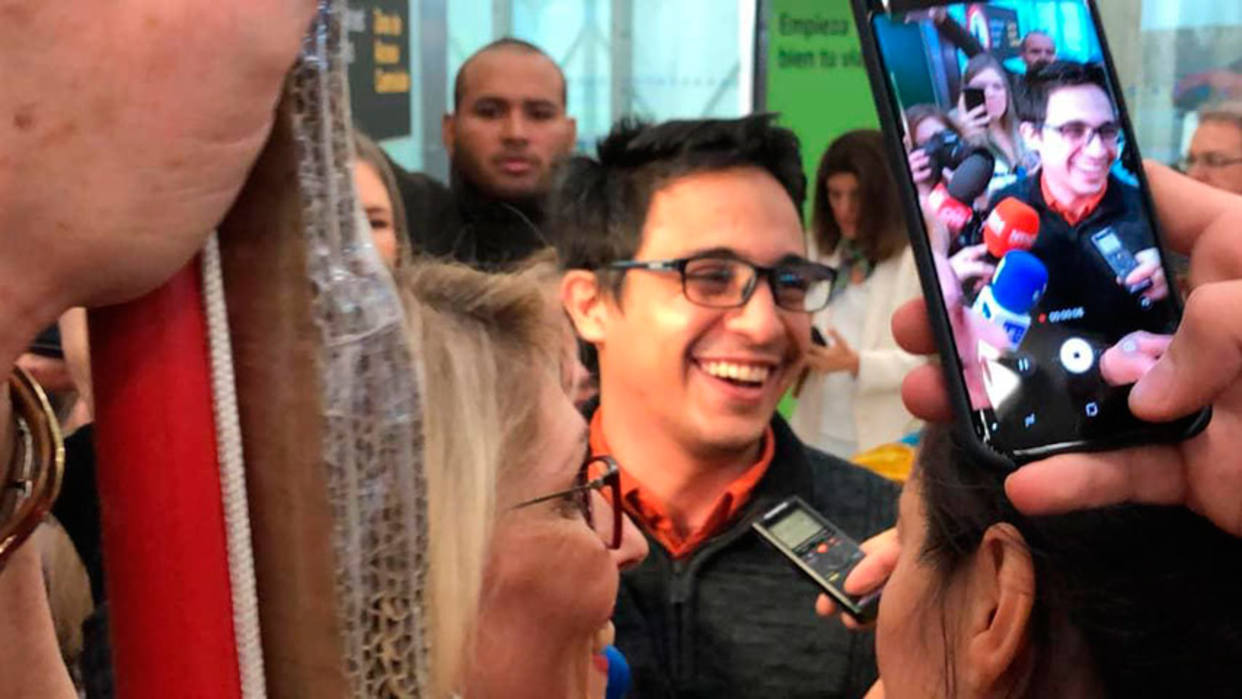
\includegraphics[width=300px]{221.jpg}%
\newline%
%
Lorent Saleh, ex preso político y activista de~los Derechos Humanos, aseguró este domingo que se está adaptando a la libertad y a la realidad de la calle.%
\newline%
%
Mediante un mensaje publicado en Instagram, Saleh señaló que el proceso de adaptación de la libertad es muy complejo después de haber estado detenido por varios años bajo un estado de terror.%
\newline%
%
"Me duele mucho no haber podido agradecerle personalmente a todas las personas que me han apoyado todo este tiempo. Estoy en deuda con Venezuela y el mundo. Espero recuperarme pronto y en los próximos días poder expresarle al mundo lo que siento y pienso en este momento", escribió en la red social.%
\newline%
%
Aseguró que seguirá comprometido con los Derechos Humanos y la libertad de conciencia en el país.%
\newline%
%
\end{document}